%!TEX root = ./ERL Industrial Robots.tex

%--------------------------------------------------------------------
%--------------------------------------------------------------------
\subsection{Object Detection Functionality}
\label{ssec:ObjectPerception}

%--------------------------------------------------------------------
\subsubsection{Functionality Description}
\label{sssec:ObjectPerceptionDescription}

This functionality benchmark evaluates robot capabilities of locating an object at a given location. One of the common tasks for service and industrial robots is to locate the object which can possibly be placed at a particular location. 
In addition to that, several secondary objects and decoys may be present at the location too. 
The robot is required to find particular objects among a set of objects and decoys. 
The target object is either included or not depending on the variation for every trial.

Objects presented to the robot in this functionality benchmark are based on the the \erlir factory scenario.
Teams are provided with a list of objects (object instances), subdivided into classes (see Section \ref{sssec:ObjectPerceptionInput}).
The objects that are used here are described in Section~\ref{sec:TestBed}.
%In this benchmark, the robot is expected to detect and estimate the object's class and identity.

%--------------------------------------------------------------------
\subsubsection{Feature Variation}
\label{sssec:ObjectPerceptionVariation}

%For this benchmark, the variation space for object features is represented by the (known) set of objects that the robot may be presented with.
For this benchmark, the variation space for objects includes: 1. A set of objects and decoys and their poses; 2. The presence of the target object [yes, no].
Furthermore, the variation space for object location is the surface of the benchmarking area where objects are located (see Section \ref{sssec:ObjectPerceptionInput}).

%--------------------------------------------------------------------
\subsubsection{Input Provided}
\label{sssec:ObjectPerceptionInput}

The set of individual objects that will actually be presented to the robot during the execution of the functionality benchmark is described in Section \ref{ssec:Objects}. 
%Object instances are subdivided into classes of objects that have one or more properties in common (``object classes''). 
%Objects of the same class share one or more properties, not necessarily related to their geometry (for instance, a class may include objects that share their application domain). 
Each object class is assigned a unique ID.

The team does not know which object instances will actually be presented to the robot during the benchmark. 
However, the team will be provided with the object information described in Section \ref{ssec:Objects}.
%
%\begin{itemize}
%\item Descriptions/models of all the object classes in the form of 3D textured models;
%\item Object classes such as Motor, KitkatMini, etc.
%\end{itemize}

Object descriptions will be expressed according to widely accepted representations, well in advance of the competition. 

%--------------------------------------------------------------------
%\subsubsection{Expected Robot Behavior or Output}
%\label{sssec:ObjectPerceptionOutput}
%
%The robot, for a set of several objects presented to it, must locate the target object. 

%\begin{itemize}
%\item Object detection: perception of the presence of an object on the table and association between the perceived object and one of the object classes (see Section \ref{sssec:ObjectPerceptionInput}).
%\item Object recognition: association between the perceived object and one of the object instances belonging to the selected class (see Section \ref{sssec:ObjectPerceptionInput}).
%
%\end{itemize}
%The following list of classes and instances of objects are going to be used in the object perception functionality benchmark:
%\begin{itemize}
%    \item Industrial
%
%    \item Chocolates
%
%    \item T-LESS
%
%\end{itemize}

%--------------------------------------------------------------------
\subsubsection{Procedures and Rules}
\label{sssec:ObjectPerceptionProcedures}

The maximum time allowed for one functionality run is 20 seconds. The time starts when the robot sends the start message to CHF until the robot sends the result message. A timeout is recorded for that run if it exceeds the allocated time and the robot must prepare for the next run.

\begin{description}
\item[Step 1] A set of target and secondary objects, decoys will be placed in front of the robot. The setup is fixed for all teams.
\item[Step 2] The robot must locate the target object represented in one of two ways:
	\begin{itemize}
	\item The 3D bounding box of the robot with respect to the robot base. In this case, the robot must provide a point cloud of the scene (transformed to the robot's base frame) corresponding to the 3D bounding box.
	\item The 2D bounding box of the objects in an image. The robot must provide the raw RGB image of the scene corresponding the 2D bounding box.
	\end{itemize}
\item[Step 3] The preceding steps are repeated until 10 runs have been completed.
\end{description}

%--------------------------------------------------------------------
\subsubsection{Communication with CFH}
\label{sssec:CommCFHObjectPerception}
For this functionality benchmark the robot does not have to control any networked device in the environment. Only the communication as described below is necessary:

\begin{description}
\item[Step 1] The robot sends a \textbf{BeaconSignal} message at least every second.
\item[Step 2] The robot waits for a \textbf{BenchmarkState} message. It starts the benchmark execution when the \emph{phase} field is equal to EXECUTION and the \emph{state} field is equal to RUNNING.
\item[Step 3] As soon as the robot has finished perceiving the object, it sends a message of type \textbf{BenchmarkFeedback} to the CFH with the required results and the \emph{phase\_to\_terminate} field set to EXECUTION. The robot should do this until the \textbf{BenchmarkState}'s \emph{state} field has changed.
\item[Step 4] The robot continues with Step 2.
\item[Step 5] The functionality benchmark ends when the \textbf{BenchmarkState}'s \emph{state} field is equal to FINISHED.
\end{description}
\noindent
The messages to be sent and to be received can be seen on the Github repository located at \cite{rockin:CFHMessages}.

%--------------------------------------------------------------------
\subsubsection{Acquisition of Benchmarking Data}
\label{sssec:ObjectPerceptionData}

Each team has to locally record the following data (at minimum):
\begin{itemize}
	\item RGB camera stream of the robot
	\item Point cloud of the scene if 3D bounding box is provided
	\item Raw RGB image if 2D bounding box is provided
\end{itemize}

The teams are encouraged to provide the dataset used for training the model.

%--------------------------------------------------------------------
\subsubsection{Scoring and Ranking}
\label{sssec:ObjectPerceptionScoring}

We use the metrics, illustrated in figure \ref{fig:ObjectDetectionMetrics}, to evaluate the performance of the robot:
\begin{itemize}
	\item True Positive (TP): the robot detects the target object when it is present
	\item False Positive (FP): the robot detects wrong object whether the target object is present or not
	\item False Negative (FN): the robot does not detect any object when the target object is present
	\item True Negative (TN): the robot does not detect any object when the target object is not present
\end{itemize} 
\begin{figure}[h!]
	\centering
	\begin{tikzpicture}	
	\node[label={\small TP}, anchor=south west,inner sep=0](B) at (-4,1) {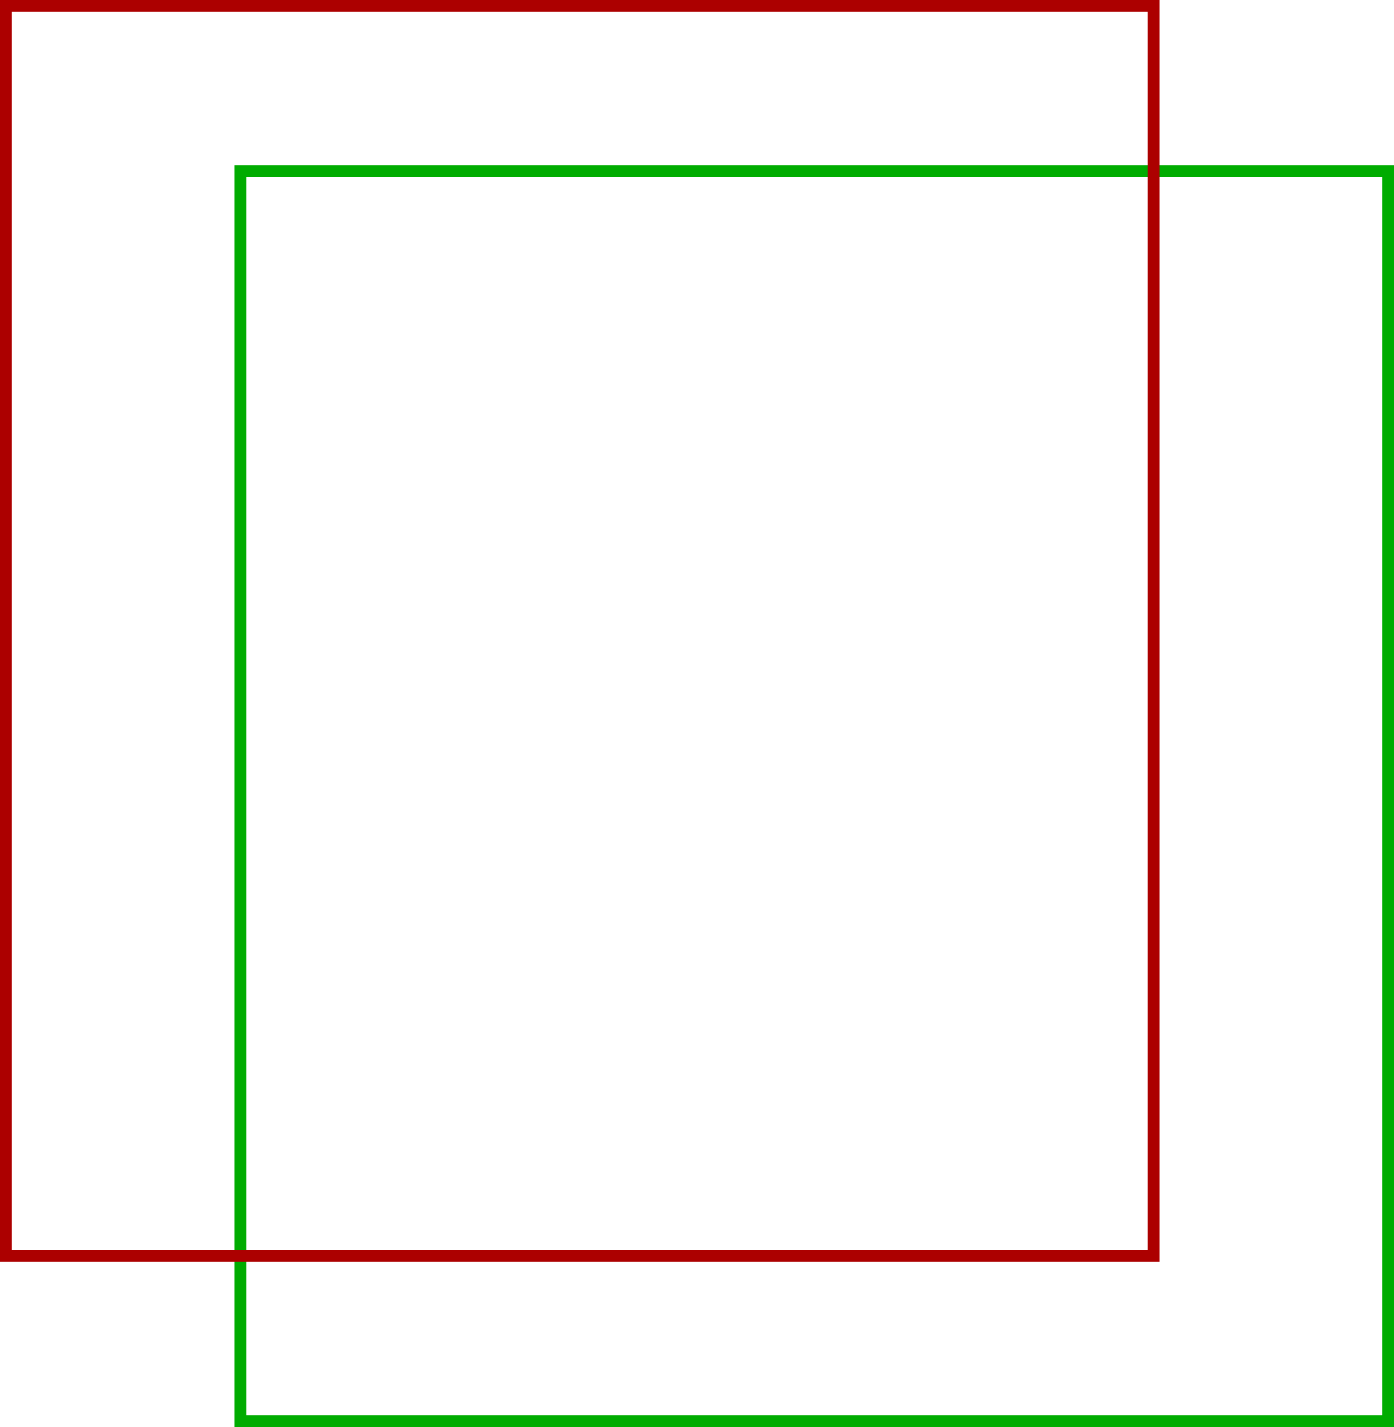
\includegraphics[width=3cm]{fig/FBM/erl/perception/sciroc-op-TP.png}};
	
	\node[label={\small FP},anchor=south west,inner sep=0](D) at (0,0.8) {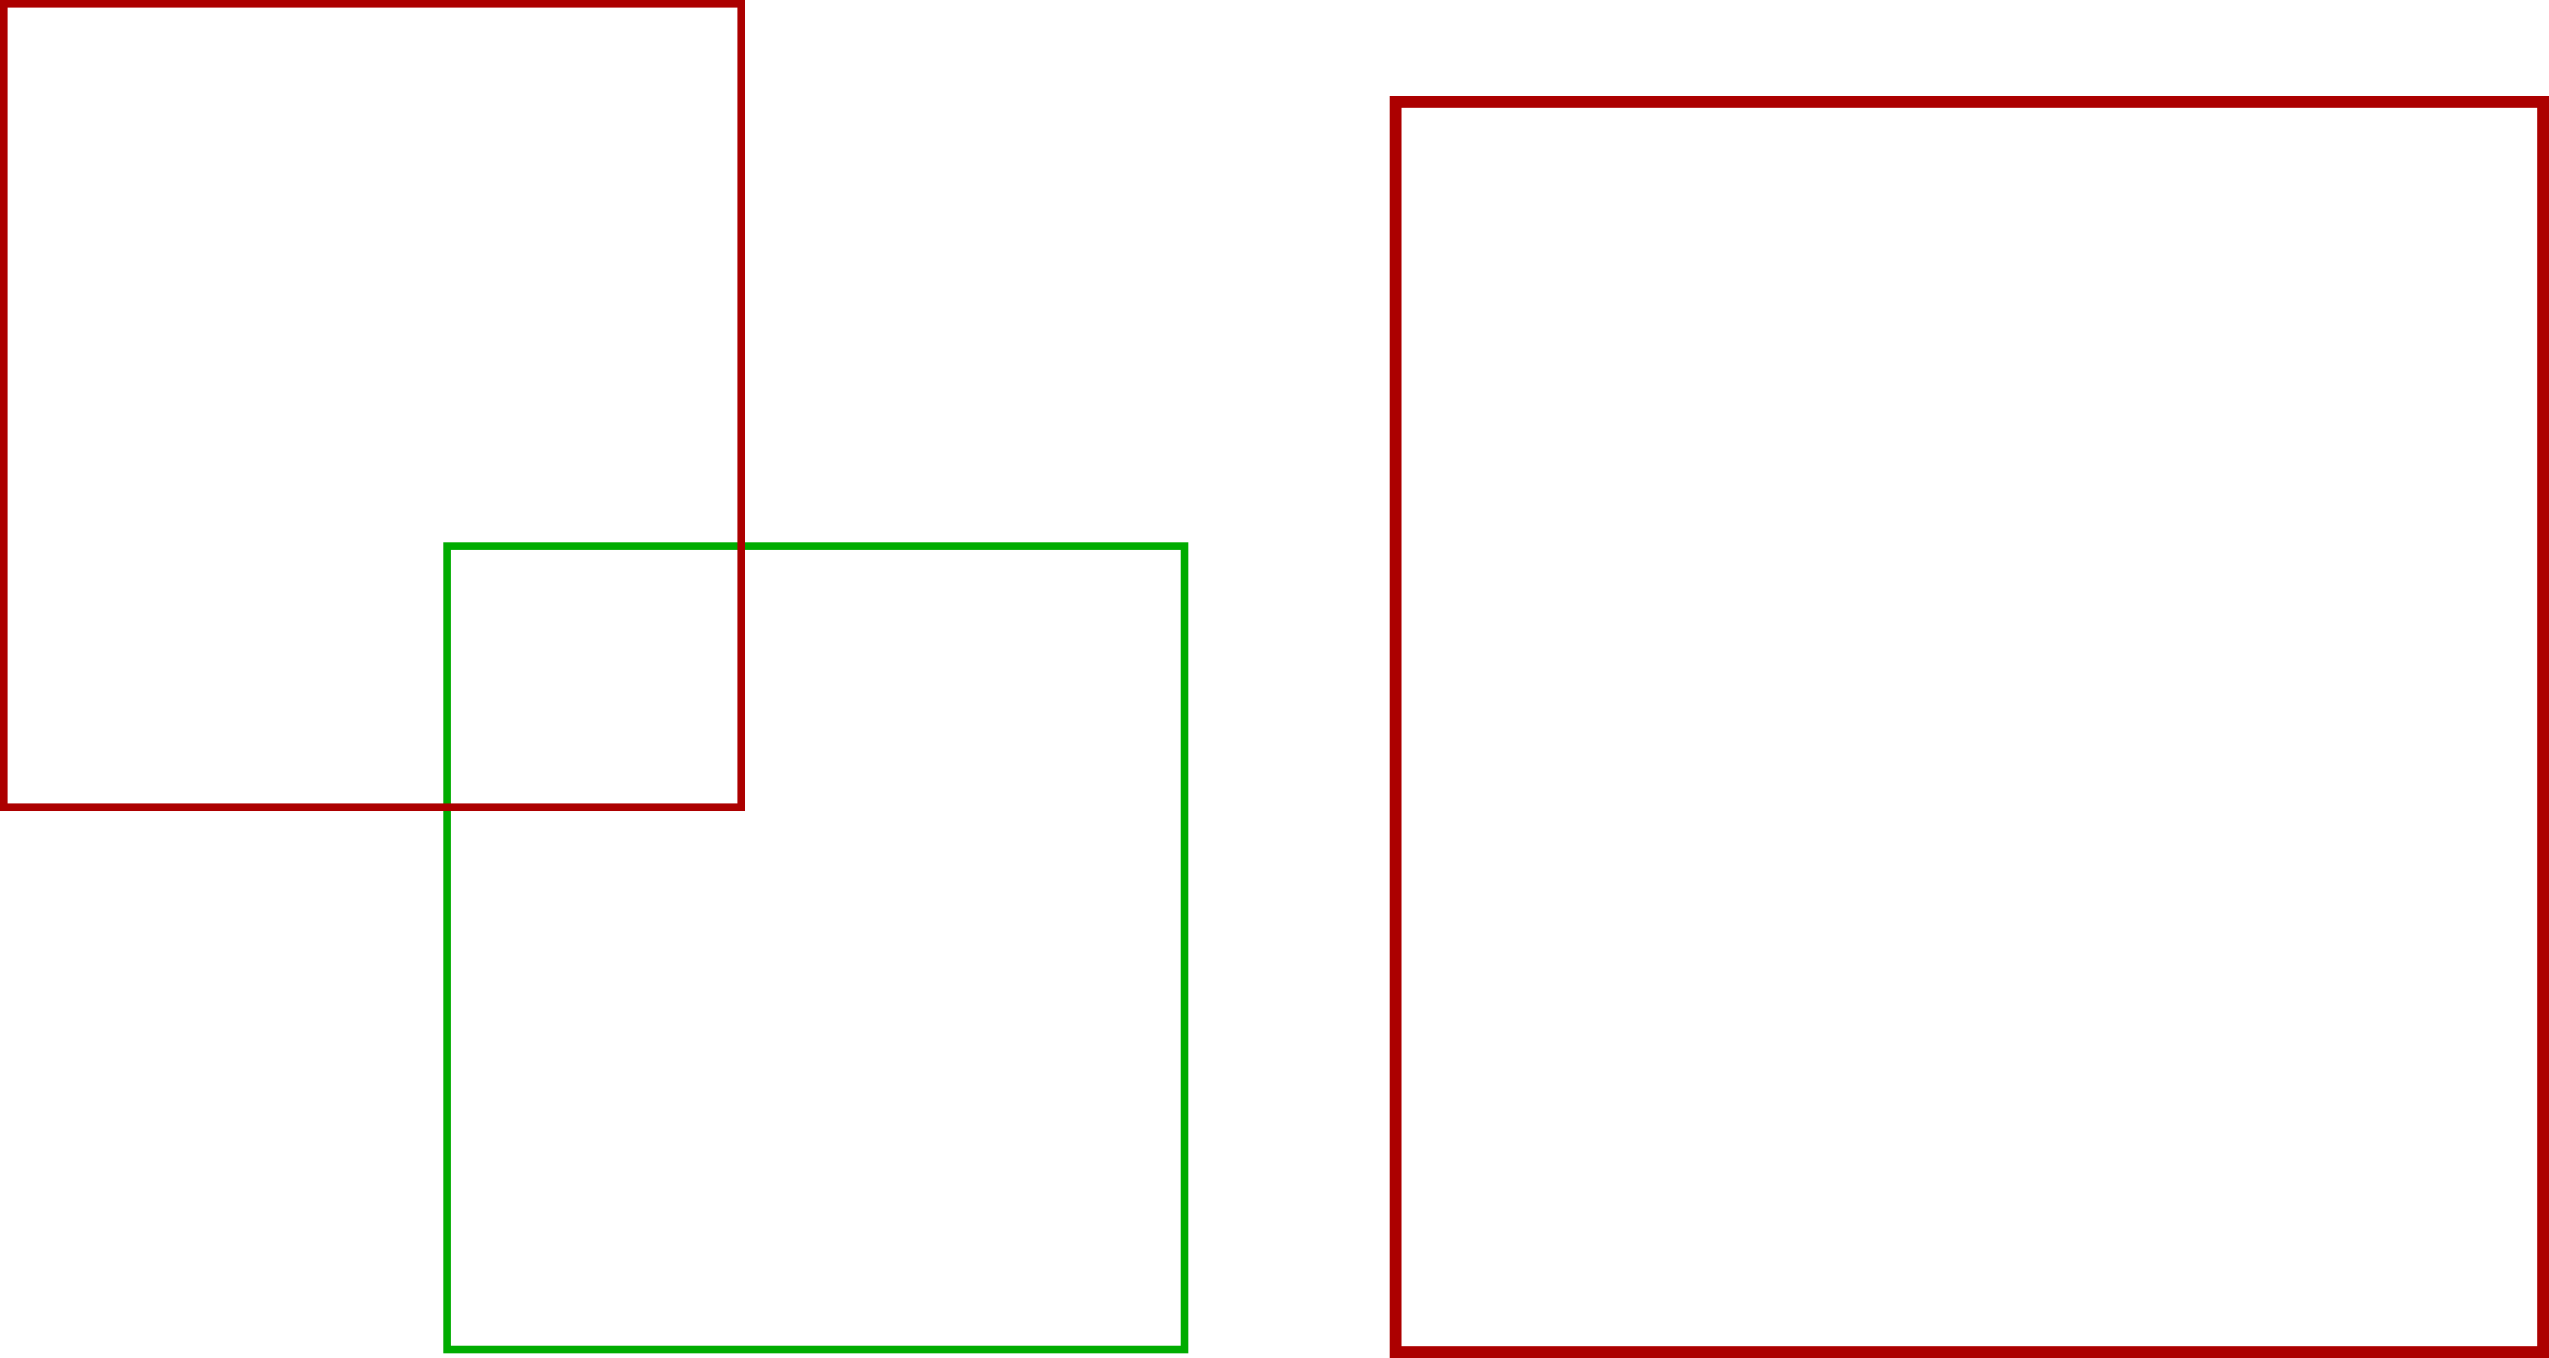
\includegraphics[width=6cm]{fig/FBM/erl/perception/sciroc-op-FP.png}};
	
	\node[label={\small FN}, anchor=south west,inner sep=0](C) at (-3.75,-3.5) {
\includegraphics[width=2.5cm]{fig/FBM/erl/perception/sciroc-op-FN.png}};
	
	\node[label={\small TN},anchor=south west,inner sep=0](E) at (1.75,-3.6) {
\includegraphics[width=2.5cm]{fig/FBM/erl/perception/sciroc-op-TN.png}};
	
	\node[anchor=south west,inner sep=0](E) at (7,3) {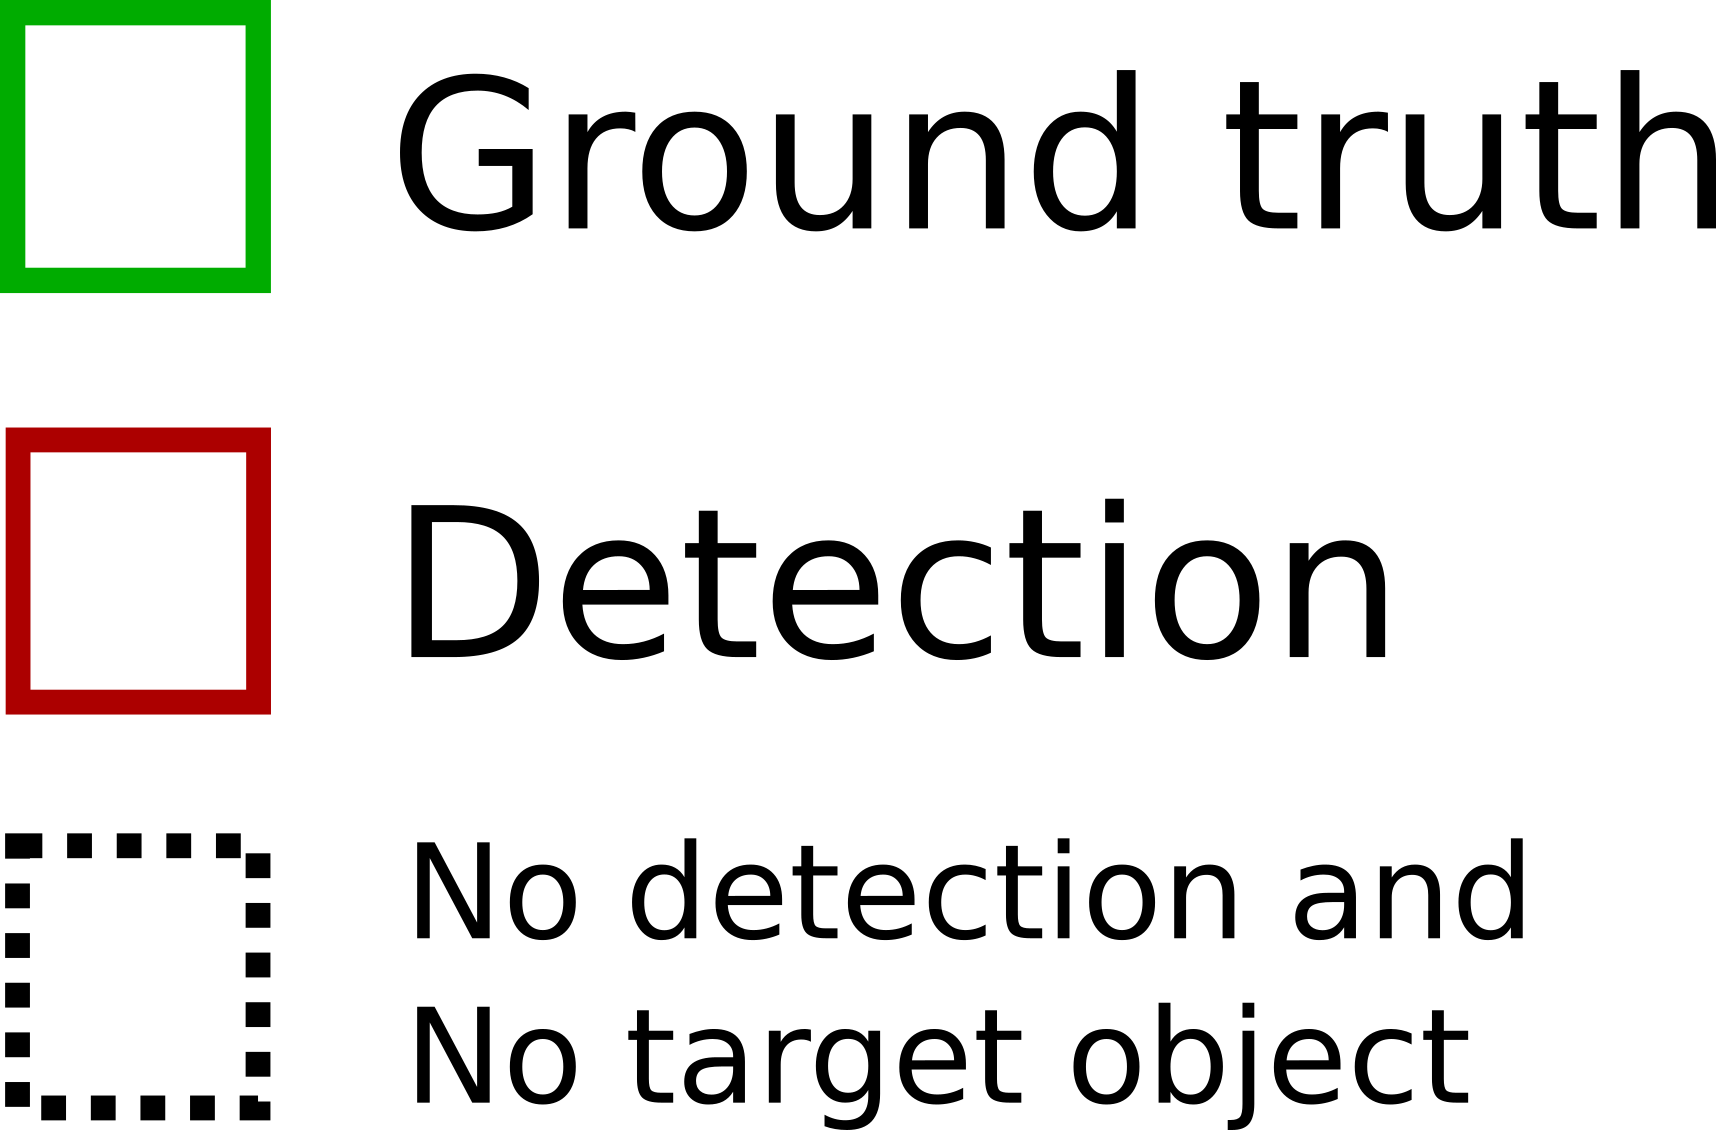
\includegraphics[width=2cm]{fig/FBM/erl/perception/sciroc-op-legend.png}};
	\end{tikzpicture}
	\caption{Metrics for object detection functionality benchmark}
	\label{fig:ObjectDetectionMetrics}
\end{figure}

For the TP and FP, the measurement is based on the degree of similarity between the ground truth and detected bounding boxes. We use the Intersection over Union (IoU),

\begin{equation}
IoU = \frac{B_{GT} \cap B_{DET}}{B_{GT} \cup B_{DET}}
\end{equation}
where $B_{GT}$ and $B_{DET}$ area the ground truth and detected bounding boxes respectively. The intersections are calculated as areas and volumes for 2D and 3D bounding boxes respectively.
In figure \ref{fig:ObjectDetectionSample} the green and red boxes show the ground truth and detected bounding boxes respectively. If the IoU is greater than a given threshold, the detection result is considered to be a true positive and otherwise it is a true negative. The same rule applies to 3D bounding boxes except that the areas will be replaced by volumes.
The IoU threshold is a configurable parameter ranging from 0.5 to 0.95 with a step size of 0.05. This approach is borrowed from the COCO challenge \footnote{https://cocodataset.org/\#detection-eval}. The TP and FP are then averaged over all IoU thresholds.


\begin{figure} [h!]
	\begin{center}
		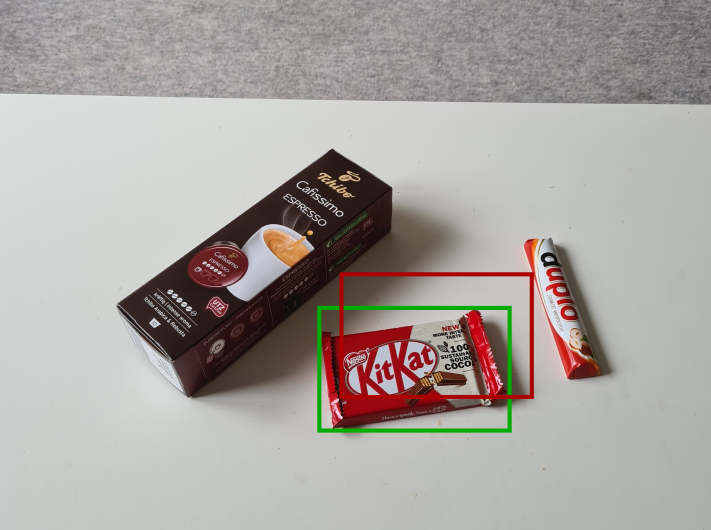
\includegraphics[width=7cm]{fig/FBM/erl/perception/sciroc-op-chocholates-bbox.png}
	\end{center}
	\caption{Object detection example: green bounding box is the ground truth and the red one is the detection.}
	\label{fig:ObjectDetectionSample}
\end{figure}

Evaluation of the performance of a robot according to this functionality benchmark is based on:
%
\begin{enumerate}
\item The sum of the TP and TN;
\item The team with the lower FP count is ranked higher;
\item The team with the lower FN count is ranked higher.
\end{enumerate}
%
The previous criteria are in order of importance; the first criterion is applied first and teams will be scored according to their accuracy, the ties are broken by using the second one still applying accuracy metrics, and in case of ties we will resort to the FN count.


%--------------------------------------------------------------------
% EOF
%--------------------------------------------------------------------
